\documentclass{ximera}

\graphicspath{{./}{thePythagoreanTheorem/}{deMoivreSavesTheDay/}{complexNumbersFromDifferentAngles/}}

\usepackage{tikz}
\usepackage{tkz-euclide}
\usetkzobj{all}
\tikzstyle geometryDiagrams=[ultra thick,color=blue!50!black]
\newcommand{\tri}{\triangle}
\renewcommand{\l}{\ell}
\renewcommand{\P}{\mathcal{P}}
\newcommand{\R}{\mathbb{R}}
\newcommand{\Q}{\mathbb{Q}}

\newcommand{\Z}{\mathbb Z}

\renewcommand{\vec}{\mathbf}
\renewcommand{\d}{\,d}



%% Egyptian symbols

\usepackage{multido}
\newcommand{\egmil}[1]{\multido{\i=1+1}{#1}{
\includegraphics[scale=.1]{egyptian/egypt_person.pdf}\hspace{0.5mm}}}
\newcommand{\eghuntho}[1]{\multido{\i=1+1}{#1}{
\includegraphics[scale=.1]{egyptian/egypt_fish.pdf}\hspace{0.5mm}}}
\newcommand{\egtentho}[1]{\multido{\i=1+1}{#1}{
\includegraphics[scale=.1]{egyptian/egypt_finger.pdf}\hspace{0.5mm}}}
\newcommand{\egtho}[1]{\multido{\i=1+1}{#1}{
\includegraphics[scale=.1]{egyptian/egypt_lotus.pdf}\hspace{0.5mm}}}
\newcommand{\eghun}[1]{\multido{\i=1+1}{#1}{
\includegraphics[scale=.1]{egyptian/egypt_scroll.pdf}\hspace{0.5mm}}}
\newcommand{\egten}[1]{\multido{\i=1+1}{#1}{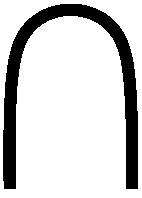
\includegraphics[scale=.1]{egyptian/egypt_heel.pdf}\hspace{0.5mm}}}
\newcommand{\egone}[1]{\multido{\i=1+1}{#1}{
\includegraphics[scale=.1]{egyptian/egypt_stroke.pdf}\hspace{0.5mm}}}
\newcommand{\egyptify}[7]{
 \multido{\i=1+1}{#1}{
\includegraphics[scale=.1]{egyptian/egypt_person.pdf}\hspace{0.5mm}}
 \multido{\i=1+1}{#2}{
\includegraphics[scale=.1]{egyptian/egypt_fish.pdf}\hspace{0.5mm}}
 \multido{\i=1+1}{#3}{
\includegraphics[scale=.1]{egyptian/egypt_finger.pdf}\hspace{0.5mm}}
 \multido{\i=1+1}{#4}{
\includegraphics[scale=.1]{egyptian/egypt_lotus.pdf}\hspace{0.5mm}}
 \multido{\i=1+1}{#5}{
\includegraphics[scale=.1]{egyptian/egypt_scroll.pdf}\hspace{0.5mm}}
 \multido{\i=1+1}{#6}{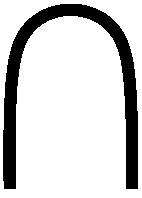
\includegraphics[scale=.1]{egyptian/egypt_heel.pdf}\hspace{0.5mm}}
 \multido{\i=1+1}{#7}{
\includegraphics[scale=.1]{egyptian/egypt_stroke.pdf}\hspace{0.5mm}}
 \hspace{.5mm}
}




\title{Limits of axioms}
\begin{document}
\begin{abstract}
In this activity, we discuss how statements can be independent of axioms.
\end{abstract}
\maketitle 



\begin{question}
Given any \textit{finite} set $S$, can you prove that the power set of
$S$ has a larger cardinality?
\end{question}

\begin{question}
Given any set $S$, can you prove that the power set of $S$ has a
larger cardinality? Hint: Attempt to ``count'' $\P(S)$ with $A_x$
where $x\in S$. Then consider $A \subset \P(S)$ where
\[
A = \{x : x \in S\text{ and } x\not\in A_x\}.
\]
\end{question}



We know that $\N$ is countable and that $\R$ is uncountable. Define:
\begin{align*}
\beth_0 &:=|\N|\\
\beth_1 &:=|\P(\N)|\\
\beth_2 &:=|\P(\P(\N))|\\
\beth_3 &:=|\P(\P(\P(\N)))|\\
        &\vdots
\end{align*}
and so on. These are \textit{beth} numbers. From our work above we see that 
\[
\beth_0 \le \beth_1 \le \beth_2 \le \beth_3 \le \cdots
\]


CAN WE PROVE BETH1 = |R|?????


On the other hand there are also \textit{aleph} numbers. Here
\[
\aleph_0 := |\N|
\]
but $\aleph_1$ is defined to be the \textit{smallest} infinite cardnal
number larger than $\aleph_0$. In general, $\aleph_n$ is the smallest
infinite cardnal number larger than $\aleph_{n-1}$. So from this
definition we find:
\[
\aleph_0 \le \aleph_1 \le \aleph_2 \le \aleph_3 \le \cdots
\]

\begin{question}
Say everything you can about the relationship between the aleph
numbers and the beth numbers.
\end{question}


In 1900 Hilbert made a list of problems to guide the mathematicicans
of the 20th Centuary. Here is the first problem on the list:

\begin{quote}
Prove the continuum hypothesis.
\end{quote}

What is this so-called continuum hypothesis? It states
\[
\aleph_1 = \beth_1 = |\R|.
\]

I speculate that finding the ``holes'' in Euclid's arguments led
Hilbert to question the validity of our own proofs. This speculation
is supported by the fact that in 1900 the second problem in Hilbert's
list of problems was:
\begin{quote}
Prove that the axioms of arithmetic are consistent.
\end{quote}

\begin{question}
What would an counterexample to this claim imply? What would an
affirmiative proof imply?
\end{question}


G\"odel!!!

Axiom of Choice.

WOP.

Zorn's Lemma.












\end{document}
